\section{Experiments and Results}

\subsection{Financial Reports Dataset}
To evaluate the performance of the RAG system, financial reports of the US companies from the FinanceBench dataset have been used \cite{Islam.20Nov2023}. FinanceBench is a new benchmarking dataset designed to assess the capabilities of LLMs in answering open-book financial questions. The questions collected are realistic and applicable to real-world financial scenarios and include complex questions that require computational reasoning to arrive at conclusive answers.

This dataset is made of 150 instances with questions and answers from 84 unique reports of 32 different companies. The dataset does not include the source documents, which we have downloaded using modified EDGAR-CRAWLER code from the \cite{Loukas.2021}. Unlike FinanceBench paper where the authors used PDF files with company reports (10-K, 10-Q, 8-K) as raw data, JSON files from the EDGAR database were downloaded and post-processed. We were able to recover only 82 documents, not including BestBuy's 2024Q2 10-Q report and Pepsico's 8-K report dated May 5, 2023 in the final dataset. 

For downloading reports EDGAR-CRAWLER's code\footnote{https://github.com/winterForestStump/thesis/tree/main/edgar-crawler-modified} was modified and used. EDGAR-CRALER is an open-source and optimized toolkit. It can crawl any report found in the SEC EDGAR database, the web repository for all publicly traded companies in the USA. Apart from downloading EDGAR filings like other standard toolkits, EDGAR-CRAWLER can also preprocess and convert them into JSON files. Two code updates were conducted to the original "extract\_items" script: additional unicode characters text cleaning steps were added (special characters were replaced with their corresponding substitutions)  and all extracted items now are saved under one 'context' key (the original code created a separate key for each item in the report).

The final JSON files contain the following information: CIK (the unique code of the company), company name, filing type (10-K for annual reports, 10-Q for quarterly report, and 8-K for current reports), filing date, period of report, SIC (Standard Industrial Classification Code), state of incorporation, location state, fiscal year, filing HTML index link, HTML filing link (link to the report in human-readable format in the EDGAR archive), complete TEXT filing link, filename, and context with the full report text. Full report text contains all the information from the 10-K, 10-Q and 8-K reports including tables data as a plain text.

Final dataset\footnote{\url{https://github.com/winterForestStump/thesis/tree/main/datasets}} contains 82 JSON files for the 32 unique companies. The length of the reports was analyzed by counting the number of words in each report\footnote{\url{https://github.com/winterForestStump/thesis/blob/main/notebooks/words_count_and_analysis.ipynb}}. The result can be seen in the histogram in \autoref{fig:word_distribution}:
\begin{figure}[h!]
\centering
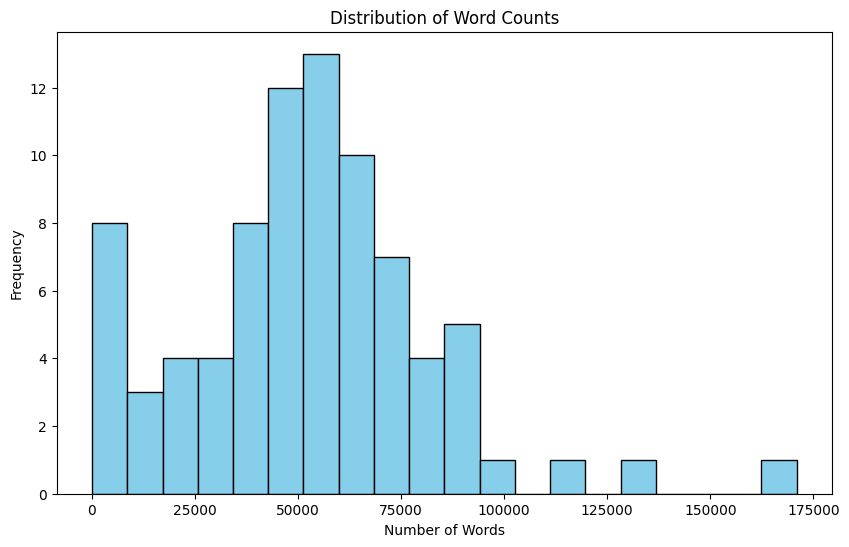
\includegraphics[width=1\textwidth]{Figures/word_distribution.png}
\caption{The size of the reports in the database}
\label{fig:word_distribution}
\end{figure}

Most reports are between 0 and 100K words long. Overall, the reports length is relatively evenly distributed: there are a few outliers (8-k reports are the smallest ones, and annual reports from the big companies are the longest).

Table \ref{table:companies} shows the list of companies, report periods and filing types that appear in the final dataset.
\begin{table}[H]
\centering
\resizebox{\textwidth}{!}{
\begin{tabular}{|c c c c|}
 \hline
 Company & Periods & Types & Total \\ [0.5ex] 
 \hline\hline
 3M & 2018, 2022, 2023Q2 & 10-K/Q & 3 \\ 
 Activision Blizzard  & 2019 & 10-K & 1 \\
 Adobe & 2015-2017, 2022  & 10-K & 4 \\
 AES Corporation & 2022 & 10-K & 1 \\
 Amazon & 2017, 2019 & 10-K & 2 \\ 
 Amcor & 2020, 2022, 2023 & 10-K/Q, 8-K & 5 \\
 AMD & 2015, 2022 & 10-K & 2 \\
 American Express & 2022 & 10-K & 1 \\
 American Water Works & 2020-2022 & 10-K & 3 \\
 Best Buy & 2017, 2019, 2023 & 10-K & 3 \\
 Block (Square) & 2016, 2020 & 10-K & 2 \\
 Boeing & 2018, 2022 & 10-K & 2 \\
 Coca-Cola & 2017, 2021, 2022 & 10-K & 3 \\
 Corning & 2020-2022 & 10-K & 3 \\
 Costco & 2021 & 10-K & 1 \\
 CVS Health & 2018, 2022 & 10-K & 2 \\
 Foot Locker & 2022 & 8-K & 2 \\
 General Mills & 2019, 2020, 2022 & 10-K & 3 \\
 Johnson\&Johnson & 2022-2023, 2022Q4, 2023Q2 & 10-K, 8-K & 4 \\
 JPMorgan & 2021Q1, 2022, 2022/23Q2 & 10-K/Q & 4 \\
 Kraft Heinz & 2019 & 10-K & 1 \\
 Lockheed Martin & 2020-2022 & 10-K & 3 \\
 MGM Resorts & 2018/20/22, 2022Q4/2023Q2 & 10-K/Q & 5 \\
 Microsoft & 2016, 2023 & 10-K & 2 \\
 Netflix & 2015, 2017 & 10-K & 2 \\
 Nike & 2018, 2019, 2021, 2023 & 10-K & 4 \\
 Paypal & 2022 & 10-K & 1 \\
 PepsiCo & 2021, 2022, 2023, 2023Q1 & 10-K, 8-K & 4 \\
 Pfizer & 2021, 2023Q2 & 10-K/Q & 2 \\
 Ulta Beauty & 2023, 2023Q4 & 10-K/Q & 2 \\
 Verizon & 2021, 2022 & 10-K & 2 \\
 Walmart & 2018-2020 & 10-K & 3 \\ 
 \hline\hline
 Total & - & - & 82 \\ [1ex] 
 \hline
\end{tabular}
}
\caption{Financial reports dataset}
\label{table:companies}
\end{table}
The annual reports have been shown to be one of the most important external documents of a company. A Form 10-K is an annual report required by the U.S. Securities and Exchange Commission (SEC), which gives a comprehensive summary of a company's financial performance \cite{USSEC.2024}. Companies with more than USD 10 million in assets and a class of equity securities that is held by more than 2000 owners must file annual and other periodic reports, regardless of whether the securities are publicly or privately traded. Following the guidance of the SEC, it should contain 4 parts and 22 Items. 

If a shareholder requests a company's Form 10-K, the company must provide a copy. In addition, most large companies must disclose on Form 10-K whether the company makes its periodic and current reports available, free of charge, on its website. Form 10-K, as well as other SEC filings may be searched at the EDGAR database on the SEC's website \cite{SECOfficeofInvestorEducationandAdvocacy.2021}.

In addition to the 10-K, which is filed annually, a company is also required to file quarterly reports on Form 10-Q. Information for the final quarter of a firm's fiscal year is included in the annual 10-K, so only three 10-Q filings are made each year. In the period between these filings, and in case of a significant event, such as a CEO departing, material cybersecurity incident or bankruptcy, a Form 8-K must be filed in order to provide up to date information \cite{SECOfficeofInvestorEducationandAdvocacy.2021}.

Laws and regulations prohibit companies from making materially false or misleading statements. Likewise, companies are prohibited from omitting material information that is needed to make the disclosure not misleading. In addition, a company’s CFO and CEO must certify to the accuracy of the 10-K and 10-Q.
The SEC does not vouch for the accuracy of a 10-K or 10-Q. The SEC sets the disclosure requirements – the topics that all companies must cover in their 10-Ks or 10-Qs, and how the information should be presented \cite{SECOfficeofInvestorEducationandAdvocacy.2021}.

The SEC staff reviews 10-Ks and 10-Qs to monitor and enhance companies’ compliance with the requirements. Both the SEC and the staff also provide interpretive advice about the disclosure requirements. The SEC staff reviews 10-Ks and may provide comments to a company where disclosures appear to be inconsistent with the disclosure requirements or deficient in explanation or clarity. The Sarbanes Oxley Act requires the SEC to review every public company’s financial statements at least once every three years. The SEC staff may review the 10-Ks and 10-Qs of certain companies more frequently \cite{SECOfficeofInvestorEducationandAdvocacy.2021}.

The length and complexity of each 10-K are company-specific, for the purposes of financial analysis and corporate valuation the following sections are where most of the time is spent: Business, Risk Factors, Management Discussion and Analysis (MDA), Financial Statements, Supplementary Disclosures. Companies are required to present their financial statements according to a set of accounting standards, conventions and rules known as Generally Accepted Accounting Principles, or GAAP. An independent accountant audits the company’s financial statements. For large companies, the independent accountant also reports on a company’s internal controls over financial reporting.


\subsection{Questions sets}
Within the framework of the present work the experiments were conducted with two lists of questions: the first list consists of 35 most common and widespread questions (for convenience we will call it Regular Questions) and the list of questions from FinanceBench dataset (FinanceBench Questions).

Regular Questions\footnote{\url{https://github.com/winterForestStump/thesis/blob/main/questions/questions_ver2.txt}} is a TXT list with 35 questions on each new line with no company names (the questions are identical for each company) regarding different topics:
\begin{enumerate}
\item Questions about the financial indicators.
\begin{itemize}
    \item The total revenue is an indicator of the overall market performance and growth: typically, a steady increase in revenue indicates healthy growth.
    \item Cost of Goods Sold (COGS) represents the direct costs attributable to the production of goods sold by the company.
    \item Gross profit margin is calculated as (Revenue - COGS) / Revenue and indicates how well the company is managing its production costs relative to its sales.
    \item Major operating expenses include selling, general, and administrative expenses, research and development costs, and other overheads.
    \item Operating income, or operating profit, reflects the company’s profitability from core operations, excluding non-operating income and expenses.
    \item Net income represents the company’s total profit after all expenses, taxes, and interest.
    \item Total outstanding debt, along with its structure and interest rates, is crucial for assessing financial risk: a well-structured debt with manageable interest rates is less risky, high levels of debt could be concerning if not matched with strong earnings.
    \item Operating cash flow is a measure of the cash generated by the company's core business activities.
\end{itemize}
\item Questions about the financial ratios. 
\begin{itemize}
    \item Earnings Per Share (EPS) measures the profitability available to each share of common stock, making it a key indicator for investors, comparing EPS with industry benchmarks provides context on the company's relative performance.
    \item Capital expenditures (CapEx) represents the company’s investment in its fixed assets, significant CapEx could indicate expansion or upgrades of facilities and equipment.
    \item The current ratio (current assets/current liabilities) and quick ratio (quick assets/current liabilities) are key indicators of the company’s short-term liquidity.
    \item Inventory levels and turnover rates provide insights into inventory management efficiency: high inventory turnover is generally favorable, indicating efficient sales and inventory management; Conversely, excess inventory may signal potential management issues.
    \item Accounts receivable turnover measures how effectively the company collects revenue: high turnover indicates efficient collection processes, while low turnover may suggest issues with credit policies or customer payment delays.
\end{itemize}
\item Questions about risks, market share, future plans and other. 
\begin{itemize}
    \item The company’s 10-K report outlines significant risks and mitigation strategies, these insights are critical for understanding potential future challenges and the company’s preparedness.
    \item Understanding the company’s market share and how it has evolved helps assess competitive positioning.
    \item The Management Discussion and Analysis (MD\&A) section provides management’s perspective on financial results, business conditions, and future outlook, it offers valuable insights into strategic priorities and operational focus.
    \item Ongoing legal proceedings can impact financial stability and reputation, understanding these issues and their potential impact is essential for risk assessment.
    \item The effective tax rate and any tax-related risks or benefits are crucial for understanding net income variability, tax strategies can significantly influence profitability.
    \item Research and Development (R\&D) spending indicates the company’s commitment to innovation: significant projects or innovations in progress can provide a competitive edge and drive future growth.
    \item Share buyback programs can signal management’s confidence in the company’s prospects. Understanding the rationale behind buybacks helps assess their impact on shareholder value.
    \item Analyzing the company's dividend history helps assess the sustainability of dividend payouts.
    \item Employee benefits and corporate culture play a significant role in attracting and retaining talent: a positive culture can drive productivity and innovation.
    \item Environmental, Social, and Governance (ESG) concerns and sustainability initiatives are increasingly important to investors and consumers.
    \item The geographic distribution of revenue provides insights into market diversification and regional performance.
    \item Managing currency risk is essential for companies operating internationally. Understanding the impact of currency fluctuations on financials helps assess economic exposure.
    \item Disclosed accounting policies and potential changes can affect financial statements.
    \item Pension obligations and contributions are important for assessing long-term financial commitments: a pension fund surplus or deficit can significantly impact financial health.
    \item Leveraging technology for operations and ongoing advancements can enhance efficiency and competitiveness.
    \item Management’s views on future growth, strategic plans, and anticipated challenges provide a road map for potential developments and market positioning.
\end{itemize}
\end{enumerate}

The second set of questions is FinanceBench Questions\footnote{\url{https://github.com/patronus-ai/financebench/blob/main/data/financebench_open_source.jsonl}}, which consists of 150 specific to the each company questions with provided ground truth answers. The questions collected are realistic and applicable to real-world financial scenarios and include complex questions that require computational reasoning to arrive at conclusive answers.


\subsection{Experiments Setup}
Google Disk (free subscription) was used to store the reports and vector database. Since executing code on CPU is very slow (some operations are 18 times slower on CPU then GPU) and using the Google virtual machine Colab Free Tier is almost impossible due to time and GPU usage limits. A monthly Google Colab Pro subscription (EUR 11.01 with VAT) was purchased, which provides a virtual machine with 100 computational units (usage rate is approximately 1.76 per hour for T4 GPU), 12.7GB system RAM, 15GB GPU RAM and 201.2GB Disk Storage.

Open-sourse libraries and frameforks were used, no API was used. HuggingFace\footnote{https://huggingface.co/} was used to access embeddings models and LLMs. The LLamaCpp\footnote{https://github.com/ggerganov/llama.cpp} framework was also used to inference with Meta's LLAMA architecture model locally. The LangChain\footnote{\url{https://https://github.com/langchain-ai/langchain/}} framework was used for creating RAG architecture with retrievals and chains.

\subsection{Database Deployment}
Annual reports are unstructured data, they cannot be stored in a pre-defined format or fit into an existing data (table-based) model. For tokenization (creating vector representation of the text) annual reports the "BAAI/bge-small-en-v1.5" embedding model from HuggingFace was used. The vectors were normalized to calculate cosine similarity between them.

Since reports are long, they should be divided into parts. For chunking 'RecursiveCharacterTextSplitter' (from LangChain library) was used. It tries to split on the default list of characters in order until the chunks are small enough. This has the effect of trying to keep all paragraphs (and then sentences, and then words) together as long as possible, as those would generically seem to be the strongest semantically related pieces of text. The number of characters in each chunk (chunk size) is 256. The LangChain library offers many other different types of text splitters: HTML splits on html specific characters, Markdown - on markdon specific characters and others. At a high level, text splitters work as following: Split the text up into small, semantically meaningful chunks (often sentences). Start combining these small chunks into a larger chunk until you reach a certain size (as measured by some function). Once you reach that size, make that chunk its own piece of text and then start creating a new chunk of text with some overlap (to keep context between chunks)\footnote{\url{https://python.langchain.com/v0.1/docs/modules/data_connection/document_transformers/}}.

The choice of the correct chunk size is not a trivial task. Firstly, there is a limitation from the maximum sequence length of the embedding model. Since bge-small-en-v1.5 model basis on BERT than the maximum sequence length is 512, so the maximum chunk size should be less than 512. Otherwise, the model applies a truncation strategy and silently ignores all tokens after 512 one. There is a trade off between 128, 256 or 512 sizes between preserving context and maintaining accuracy. Smaller chunks may provide better accuracy but lost context. The best way is by exploring a variety of chunk sizes, including smaller chunks (e.g., 128 or 256 tokens) for capturing more granular semantic information and larger chunks (e.g., 512 or 1024 tokens) for retaining more context. But that wasn't in the scope of our paper. In order to maintain a balance between preserving context and accuracy we decided to use a  'ParentDocumentRetriever' (from LangChain library). The 'ParentDocumentRetriever' splitts and storing small chunks of data (child chunks). During retrieval, it first fetches the small chunks but then looks up the parent ids for those chunks and returns those larger documents (parent chunks). For child chunk we have chosen the size of 256 tokens (for the accuracy) and for the parent chunks the size of 2000 (to preserve the context). 

For storing vector embeddings we use collections in ChromaDB. We have created 3 collections with the same vector, but with different distance functions: euclidean distance (l2), inner product, cosine similarity. ChromaDB uses distance function to search through the database and compute the similarity. Our first experiments are about to compare all 3 functions and choise the best one to work with in future. 

After the collections were created we used a JSONLoader (from LangChain library) to load reports in JSON format. While loading we also define the metadata for every chunk with some useful information such as CIK, company name, filing type and date, period of report, state location, fiscal tear end, html filing link and filename. We will use company name in future experiments for filtering queries during the database search stage. All other metadata keys may also be used in future to enhance retrieval part of the system.

In total there are 17561 parent chunks which are divided into 356275 child chunks, which are stored in every collection in the Chroma database. Estimated storage for every collection can be calculated by formula \cite{QuentinAnthonyStellaBidermanHaileySchoelkopf.2023}: Storage = Dimensionality of the vectors x 4 bytes x Number of documents (chunks).

384 (dimension of the vectors) x 4 (bytes) x 356275 (chunks) = 547 Mb. Every collection additionally has ids, metadata and indexes.


\subsection{Initial Experiments with RAG Architectures}
In this section the results of the first experiments with different RAG architectures are provided. Some of the conclusions from the experiments will be used in the following subsections.

Using the embedding model the report's texts were tokenized into vectors, splitted with 'RecursiveCharacterTextSplitter' into small (256 tokens) and big (2000 tokens) chunks and stored into the ChromaDB collection with a default Euclidean distance function. Questions from the Regular Questions were asked about 5 companies (Nike, CocaCola, 3M, Adobe, General Mills). Each question was augmented with the company's name. 'ParentDocumentRetriever' searched for the most similar chunks to the questions in the database and returned them as the context to the LLM.

For answering the questions Llama-2-7b-Chat-GPTQ model from HuggingFace was used\footnote{\url{https://huggingface.co/TheBloke/Llama-2-7B-Chat-GPTQ}}. Llama 2 is an auto-regressive language model that uses an optimized transformer architecture, was trained between January 2023 and July 2023. The model had following hyper-parameters: temperature (controls randomness of predictions; for use cases that need to always be factually grounded, very low temperature values are recommended, while more creative tasks can benefit from higher temperatures.) = 0.0001, max\_new\_tokens (number of generated tokens) = 2048, top\_p (manages randomness) = 0.9, repetition\_penalty (discourages repetitive or redundant output) = 1.1. The model after receiving the retrieved documents as context, provided responses for every question\footnote{\url{https://github.com/winterForestStump/thesis/blob/main/notebooks/experiment_llama2_chain_filter_flashrerank.ipynb}}. 

The LLM's system prompt for the model was the following: "Use the following information from company annual reports and answer the question at the end. If the answer is not contained in the provided information or if there is NO context at all, say "The answer is not in the context". 

The responses were manually evaluated. Two binary questions were asked to each question-answer pairs: 'Is the context relevant to the company?" and "Is the context relevant to the question?" to to assess the quality of the system retrieval process. The answers to the questions are binary - 'Yes' and 'No'. Each 'Yes' answer corresponds to 1, and each 'No' answer corresponds to 0. Later, all results for each question are summed and the usual average is calculated: (number of positive answers)/ (total number of answers).

Experiments were conducted with the following architectures: 1) Naive (simple) RAG and 2) Naive RAG plus metadata filtering during the retrieval stage, when company's name was provided for the search filter to the 'ParentDocumentRetriever':
\begin{verbatim}
search_kwargs = {'filter': {'company': COMPANY_NAME}}
\end{verbatim}
The results of the experiments are shown in the \autoref{table:initial}.\\ 

\begin{table}[h!]
\centering
\resizebox{\textwidth}{!}{
\begin{tabular}{|c|c|c|}
\hline
Metric & Naive & Naive + Filter \\ [0.5ex] 
\hline
Is the context relevant to the company? & 0.743 & 1.000 \\ 
Is the context relevant to the question?  & 0.600 & 0.657 \\[1ex] 
\hline
\end{tabular}
}
\caption{Results of the initial experiments}
\label{table:initial}
\end{table}

The initial experiments with different Retrieval-Augmented Generation (RAG) architectures yielded several key insights that will inform future analysis:
\begin{enumerate}
\item Using a company name filter significantly improved the relevance of the retrieved context to the company, achieving 100\% accuracy. This approach also enhanced the context's relevance to the question, increasing the score from 0.600 to 0.657.
\item For effective filtering, it is crucial to use the exact company name as specified in the metadata. This ensures precise and relevant document retrieval.
\item The retrieval process did not incorporate date filtering, resulting in the retrieval of identical chunks from documents across different dates. This suggests that date-specific relevance was not considered in the initial experiments.
\item The responses generated by the Llama-2-7b-Chat-GPTQ model were noted to be unstable and unpredictable, indicating a need for further refinement in handling the retrieved context.
\item The results are based on experiments conducted with five companies (Nike, CocaCola, 3M, Adobe, General Mills). Therefore, additional testing with a broader range of companies is necessary to generalize the findings.
\end{enumerate}

For future experiments, applying metadata filtering is essential to maintain high relevance and accuracy. 

\subsection{Retrieval Experiments}
\subsubsection{Distance Functions}
There are three primary distance functions: L2 or Euclidean distance, cosine similarity, and inner product, which can be used by a database for similarity search in vector storage.  The question of using different functions depends on the nature of the data and the task at hand.

Euclidean distance is primarily used when the magnitudes of the vectors differ, and the primary concern is the actual distance or semantic distance between words in space. In contrast, cosine similarity focuses on the difference in semantic orientation between vectors. When vectors are normalized, cosine similarity becomes equivalent to the inner product. The inner product itself combines aspects of both Euclidean distance and cosine similarity. It is faster than cosine similarity and offers greater flexibility.

The mathematical formulas for different distance functions are in the \autoref{table:formulas}.
\begin{table}[h!]
\renewcommand{\arraystretch}{2.5}
\centering
\begin{tabular}{|>{\centering\arraybackslash}m{4cm}|>{\centering\arraybackslash}m{9cm}|}
\hline
\textbf{Measure} & \textbf{Formula} \\ \hline
\textbf{Euclidean Distance} & \( d(\mathbf{a}, \mathbf{b}) = \sqrt{\sum_{i=1}^{n} (a_i - b_i)^2} \) \\ \hline
\textbf{Inner Product} & \( \mathbf{a} \cdot \mathbf{b} = \sum_{i=1}^{n} a_i b_i \) \\ \hline
\textbf{Cosine Similarity} & \( \cos(\theta) = \frac{\sum_{i=1}^{n} a_i b_i}{\sqrt{\sum_{i=1}^{n} a_i^2} \sqrt{\sum_{i=1}^{n} b_i^2}} \) \\ \hline
\end{tabular}
\caption{Distance Functions Formulas}
\label{table:formulas}
\end{table}

Distance function for the collection in ChromaDB cannot be changed after the collection is created. In order to chose the best distance function to use, the experiments were conducted on 3 identical collections of vectors (embedded chunks of financial reports) with 3 different distance functions.

In preparing the experiments, an issue arose about the wording of the questions, namely the need to use the company name in the question. Intuitively, realizing that not every chunk contains the name of the company of interest, and the use of the company name in the question may worsen the quality of the semantic search. But for the final decision, it was decided to experiment with two approaches:
\begin{enumerate}
\item The first approach does NOT include the company name in the question;
\item The second approach is that each question contains the company name.
\end{enumerate}

During the experiments 35 questions from the Regular Questions set were asked to the 3 collections (with different distance functions: cosine similarity, inner product, l2) about 13 random companies from the database deployed ('COCA COLA CO', 'AMAZON COM INC', 'PayPal Holdings, Inc.', 'GENERAL MILLS INC', 'Walmart Inc.', 'PEPSICO INC', 'Kraft Heinz Co', 'Amcor plc', 'Square, Inc.', '3M CO', 'MICROSOFT CORP', 'Ulta Beauty, Inc.', 'AES CORP') in one run with 2 approaches (with company name in the question and without). In total 78 (2 approaches x 13 companies x 3 distance functions) retrieval runs\footnote{\url{https://github.com/winterForestStump/thesis/blob/main/retrieval/Retrievals_approaches.ipynb}} were conducted. Every run provides 70 question-context pairs: 2 the most relevant parent chunks to each of 35 questions, saved as JSON files\footnote{\url{https://github.com/winterForestStump/thesis/tree/main/retrieval/retrievals}}.

To evaluate the results of the retrievals the "Phi-3-mini-4k-instruct-fp16.gguf" model was utilized, a GGUF format for the Phi-3-Mini-4K-Instruct model from Microsoft. The GGUF\footnote{\url{https://github.com/ggerganov/ggml/blob/master/docs/gguf.md}} format is specially designed to store inference models and perform well on consumer-grade computer hardware. 

To run the model locally the LLamaCpp with temperature (is used to control the generation randomness) equals 0 and context window (the maximum number of context tokens) equals 4096 was utilized. The model was provided with question and the retrieved context for every approach and distance function and was asked to evaluate the relevance. For each approach, the prompt templates differed only in the input variable names: approach 1 does not include the company name in the question, and the input variable name is 'question'; approach 2 includes the company name in the question, and the input variable name is 'question\_name'. 

The assistant part of the prompt is the same for both approaches: "You are a grader assessing relevance of a retrieved document to a user question. If the document contains keywords related to the user question, grade it as relevant. It does not need to be a stringent test. The goal is to filter out erroneous retrievals. Give a binary score 'yes' or 'no' score to indicate whether the document is relevant to the question. Provide the binary score as a JSON with a single key 'score' and no preamble or explanation."

For every question-document pair, the model provided binary answers: 'Yes' if the document contains information relevant to the question, or 'No' if the document does not contain information related to the question. The final score was calculated as an average from the model's responses: (Total number of "Yes" answers) / (Total number of all answers). The average similarity score was calculated for each approach and distance function\footnote{\url{https://github.com/winterForestStump/thesis/blob/main/retrieval/Retrievals_approaches_evaluation_phi3.ipynb}}.

The final results are presented in the table. The average score for every approach is in fact a precision (the fraction of relevant instances among the all retrieved instances): 
\[
\text{Precision} = \frac{\#(\text{relevant items retrieved})}{\#(\text{retrieved items})} = P(\text{relevant} \mid \text{retrieved})
\]

It is impossible to calculate recall, which is the fraction of relevant instances that were retrieved, due to the unlabeled dataset and the absence of ground truth context.

The final results for both approaches and all of the distance functions are in the \autoref{table:scores}:\\
\begin{table}[h!]
\renewcommand{\arraystretch}{2.5}
\centering
\begin{tabular}{|>{\centering\arraybackslash}m{4cm}|>{\centering\arraybackslash}m{3cm}|>{\centering\arraybackslash}m{3cm}|}
\hline
\textbf{Measure} & \textbf{Approach 1} & \textbf{Approach 2}\\ \hline
\text{Euclidean Distance} & \textbf{0.5723} & 0.3688 \\ \hline
\text{Inner Product} & 0.5671 & 0.3571 \\ \hline
\text{Cosine Similarity} & 0.5716 & 0.3794 \\ \hline
\end{tabular}
\caption{Average scores for different approaches and distance functions}
\label{table:scores}
\end{table}

Approach 1, without mentioning the company name in the questions, shows significantly better results. This confirms the initial intuition that not every small (or even large) text chunk contains a mention of the company name, which makes the question and the text part closer in meaning (with a better similarity coefficient). 

The average scores of distance functions in different approaches are quite close to each other, but the best result is Eucleadian Dicstance (L2). 

Important to note, that in the experiments the normalized data was used. The results of some researches demonstrate that the normalization of the full dataset, may lead to biased results, surprisingly, for the worse, and Euclidean distance showed not the best results \cite{Barboza.30Jun2023}.

To further analyze which questions caused the most difficulty in the document retrieval phase, the Approach 1 data for all three distance functions ere analyzed together (since they showed nearly identical results) for each of the 35 questions\footnote{\url{https://github.com/winterForestStump/thesis/blob/main/retrieval/approach_1_combined_analysis.ipynb}}:
\newcolumntype{L}[1]{>{\raggedright\arraybackslash}p{#1}}
\begin{longtable}{L{0.6\textwidth}rrr}
\toprule
question & total & correct & percentage,\% \\
\midrule
\endfirsthead
\toprule
question & total & correct & percentage,\% \\
\midrule
\endhead
\midrule
\endfoot
\endlastfoot
What does the company foresee in terms of future growth and challenges and are there any strategic plans outlined for the upcoming years? & 74 & 71 & 95 \\
What is the effective tax rate for the company? & 73 & 70 & 95 \\
Are there any ongoing legal proceedings against the company? & 73 & 68 & 93 \\
What is the company's operating income and how does it compare to the previous years? & 68 & 61 & 89 \\
What potential impact could legal issues have on the business of the company? & 77 & 69 & 89 \\
Are there any tax-related risks or benefits for the company mentioned? & 75 & 66 & 88 \\
Who are the company's main competitors and how does the company differentiate itself? & 66 & 56 & 84 \\
How does the company manage currency risk and are there impacts on financials due to currency fluctuations? & 71 & 58 & 81 \\
What is the total revenue generated by the company and how has the revenue changed over the past few years? & 67 & 54 & 80 \\
What are the company's critical accounting policies disclosed and how might changes in these policies affect financial statements? & 70 & 56 & 80 \\
How does the company's management view the company performance? & 70 & 55 & 78 \\
What is the company's cash flow generated from operations and are there any notable trends or fluctuations? & 69 & 54 & 78 \\
Has the company engaged in any share buyback programs and if yes what is the rationale behind such actions? & 68 & 53 & 77 \\
What is the company's net income for the current fiscal year and how has net income trended over the past few years? & 72 & 53 & 73 \\
What employee benefits does the company offer? & 71 & 52 & 73 \\
What are the company's key risks mentioned in the 10-K and how does the company plan to mitigate these risks? & 66 & 46 & 69 \\
What are the company's major operating expenses and how have these expenses changed over time? & 75 & 50 & 66 \\
How much has the company invested in capital expenditures and are there any significant projects underway? & 68 & 43 & 63 \\
How does the company leverage technology for its operations and are there ongoing technological advancements? & 70 & 43 & 61 \\
What is the company's geographic breakdown of revenue and are there any notable trends or shifts? & 76 & 44 & 57 \\
How does the company address Environmental, Social, and Governance (ESG) concerns and are there any sustainability initiatives in place? & 72 & 41 & 56 \\
What is the company's total outstanding debt, how is the debt structured, and what are the interest rates? & 76 & 43 & 56 \\
What are the company's key insights provided in the Management Discussion and Analysis (MD\&A) section? & 71 & 39 & 54 \\
What are the company's pension obligations and contributions and is there a pension fund surplus or deficit? & 76 & 40 & 52 \\
How much is spent on research and development by the company? & 72 & 31 & 43 \\
What is the company's dividend history and how sustainable are the dividend payouts? & 76 & 30 & 39 \\
What is the company's gross profit margin, and how has it evolved? & 72 & 21 & 29 \\
What innovations or projects are currently in progress in the company? & 72 & 21 & 29 \\
How much inventory does the company hold and are there any signs of inventory management issues? & 68 & 18 & 26 \\
What is the company's cost of goods sold (COGS) and how does the COGS compare to the total revenue? & 70 & 11 & 15 \\
What is the company's earnings per share and how does it compare to industry benchmarks? & 77 & 10 & 12 \\
How is the company's corporate culture described? & 77 & 8 & 10 \\
What is the company's market share in its industry and how has it changed over the years? & 78 & 4 & 5 \\
What is the company's accounts receivable turnover and are there any concerns regarding receivables aging? & 64 & 1 & 1 \\
What is the company's current ratio and quick ratio and how do these ratios compare to industry averages? & 70 & 0 & 0 \\
\hline
Total & 2510 & 1440 & 57 \\
\hline
\caption{The results for Approach 1 and for all 3 distance metrics} \\
\end{longtable}

The 'total' number is the number of retrieved context from the ChromaDB using the similarity scores, the 'correct' number shows the number of times when the LLM answered that the provided context is relevant to the question. The 'percentage' column is an average score, showing the accuracy. The maximum number of "total" number is 78 (2 the most relevant chunks x 13 companies x 3 distance functions). Approach 1 received a total of 2510 question-answer-evaluation pairs, this is less than 2,730 (78 x 35 questions) because not always two the most similar chunks were received for each question, but sometimes for some questions only one, and because of 15 evaluation errors. 

Based on the data presented in the table, we can draw several conclusions and inferences about the effectiveness of document retrieval according to the given questions:
\begin{enumerate}
\item Questions related to future growth, challenges, strategic plans, and effective tax rates exhibit high accuracy (95\%). This suggests that these types of information are clearly and consistently presented in documents, making them easier to retrieve accurately.
\item Questions about legal proceedings, operating income, and potential legal impacts also have high accuracy (89-93\%). Legal data seems to be well-documented in company reports, aiding retrieval accuracy.
\item Questions on employee benefits and key risks show lower accuracy (69-73\%). These topics may be detailed in various sections or be subject to more interpretative reporting, complicating accurate retrieval. 
\item Questions about operating expenses and capital expenditures have about 63-66\% accuracy. This suggests variability in how these figures are reported or labeled in documents.
\item Questions about the geographic breakdown of revenue, ESG initiatives, pension obligations and R\&D spending have relatively low accuracy (43-57\%). These topics may not be covered comprehensively in standard financial documents, leading to difficulty in retrieval.
\item Questions about dividend history and gross profit margin exhibit very low accuracy (29-39\%). These details can be scattered or calculated differently, challenging straightforward retrieval.
\item Questions on ongoing innovations, inventory management, and cost of goods sold (COGS) show poor retrieval performance (15-29\%). These topics often involve specific details that may not be explicitly outlined in main sections.
\item Questions regarding earnings per share, corporate culture, and market share are highly inaccurate (5-12\%). These topics might not be directly addressed in standard documents or require a level of analysis not easily retrievable through basic similarity metrics.
\item Questions on current and quick ratios, and accounts receivable turnover show near-zero accuracy (0-1\%). Such financial metrics may just absent in most of the reports, they require calculation from multiple financial sections, which is difficult with simple retrieval approaches.
\end{enumerate}

\subsubsection{Re-Ranker}
Up to this point, we've employed an embedding model to locate the top 2 relevant chunks within the database. We've kept the number of chunks (top\_k) small due to the limited context length of the LLM. However, this approach assumes that the top 2 retrieved chunks are the most relevant and correctly ordered. But the problem may arise when some relevant chunks are ranked much lower than others. In this section, we introduce re-ranking. This allows us to broaden our search within the database by retrieving more segments (top\_k = 10) and then reorder them based on the highest 2 ranking scores.

In the next stage of the analysis, for the best approach 1 and Eucleadian distance (l2) distance function, we conducted retrieval experiments with using a re-ranker - BAAI/bge-reranker-v2-m3. Different from embedding model, re-ranker uses question and document as input and directly output similarity instead of embedding. We asked the system the same 35 questions according to the approach 1 (without company names in the question) about the same 13 companies. But now 'ParentDocumentRetriever' retrieved top 10 documents (top\k = 10) and after that Re-ranker recomputed the scores and leave only 2 the best of them with the highest similarity score\footnote{\url{https://github.com/winterForestStump/thesis/blob/main/retrieval/Retrievals_l2_with_reranker.ipynb}}. Again, as in the previous experiments the company names were directly putted into the search filter of the database. As a result we have 13 JSON files with the question-content pairs\footnote{\url{https://github.com/winterForestStump/thesis/tree/main/retrieval/retrievals/reranked}}.

After we conducted the same as before evaluation of the retrieved documents relevance to the question with using "Phi-3-mini-4k-instruct-fp16.gguf" model and calculated the average score (number of 'Yes' answers divided by the number of total question-answers pairs)\footnote{\url{https://github.com/winterForestStump/thesis/blob/main/retrieval/Retrievals_reranked_l2_evaluation_phi3.ipynb}}.

The results from the \autoref{table:results} show the significant improvement in relevance of the context to the question with the average score of 0.7305.
\begin{table}[H]
\renewcommand{\arraystretch}{2.5}
\centering
\begin{tabular}{|>{\centering\arraybackslash}m{4cm}|>{\centering\arraybackslash}m{3cm}|>{\centering\arraybackslash}m{3cm}|}
\hline
\textbf{Measure} & \textbf{Naive} & \textbf{Re-Ranker}\\ \hline
\text{L2, Approach 1} & 0.5723 & \textbf{0.7305} \\ \hline
\end{tabular}
\caption{Comparison of the results without and with using Re-ranker}
\label{table:results}
\end{table}

In order to further analyze how the re-ranker influenced to the particular questions we present the data for Approach 1 Euclidean Distance with Re-ranker\footnote{\url{https://github.com/winterForestStump/thesis/blob/main/retrieval/reranker_combined_analysis.ipynb}}:

\newcolumntype{L}[1]{>{\raggedright\arraybackslash}p{#1}}
\begin{longtable}{L{0.6\textwidth}rrr}
\toprule
question & total & correct & percentage,\% \\
\midrule
\endfirsthead
\toprule
question & total & correct & percentage,\% \\
\midrule
\endhead
\midrule
\endfoot
\endlastfoot
Are there any ongoing legal proceedings against the company? & 10 & 10 & 100 \\
Are there any tax-related risks or benefits for the company mentioned? & 10 & 10 & 100 \\
What is the company's cash flow generated from operations and are there any notable trends or fluctuations? & 8 & 8 & 100 \\
What is the company's cost of goods sold (COGS) and how does the COGS compare to the total revenue? & 2 & 2 & 100 \\
What is the company's geographic breakdown of revenue and are there any notable trends or shifts? & 4 & 4 & 100 \\
What are the company's critical accounting policies disclosed and how might changes in these policies affect financial statements? & 13 & 13 & 100 \\
What is the company's operating income and how does it compare to the previous years? & 7 & 7 & 100 \\
What is the effective tax rate for the company? & 8 & 8 & 100 \\
What is the total revenue generated by the company and how has the revenue changed over the past few years? & 10 & 10 & 100 \\
What potential impact could legal issues have on the business of the company? & 13 & 13 & 100 \\
What does the company foresee in terms of future growth and challenges and are there any strategic plans outlined for the upcoming years? & 13 & 13 & 100 \\
How does the company manage currency risk and are there impacts on financials due to currency fluctuations? & 12 & 11 & 91 \\
Has the company engaged in any share buyback programs and if yes what is the rationale behind such actions? & 12 & 11 & 91 \\
What is the company's total outstanding debt, how is the debt structured, and what are the interest rates? & 7 & 6 & 85 \\
How does the company's management view the company performance? & 12 & 10 & 83 \\
How does the company leverage technology for its operations and are there ongoing technological advancements? & 11 & 9 & 81 \\
What is the company's net income for the current fiscal year and how has net income trended over the past few years? & 5 & 4 & 80 \\
Who are the company's main competitors and how does the company differentiate itself? & 10 & 8 & 80 \\
How much has the company invested in capital expenditures and are there any significant projects underway? & 9 & 7 & 77 \\
What employee benefits does the company offer? & 13 & 10 & 76 \\
What are the company's major operating expenses and how have these expenses changed over time? & 11 & 8 & 72 \\
What are the company's pension obligations and contributions and is there a pension fund surplus or deficit? & 7 & 5 & 71 \\
What are the company's key risks mentioned in the 10-K and how does the company plan to mitigate these risks? & 10 & 7 & 70 \\
What are the company's key insights provided in the Management Discussion and Analysis (MD\&A) section? & 13 & 9 & 69 \\
How much inventory does the company hold and are there any signs of inventory management issues? & 9 & 6 & 66 \\
What is the company's dividend history and how sustainable are the dividend payouts? & 11 & 7 & 63 \\
What innovations or projects are currently in progress in the company? & 13 & 8 & 61 \\
How does the company address Environmental, Social, and Governance (ESG) concerns and are there any sustainability initiatives in place? & 12 & 7 & 58 \\
How much is spent on research and development by the company? & 11 & 5 & 45 \\
What is the company's gross profit margin, and how has it evolved? & 11 & 4 & 36 \\
What is the company's earnings per share and how does it compare to industry benchmarks? & 4 & 1 & 25 \\
How is the company's corporate culture described? & 9 & 2 & 22 \\
What is the company's market share in its industry and how has it changed over the years? & 11 & 1 & 9 \\
What is the company's accounts receivable turnover and are there any concerns regarding receivables aging? & 7 & 0 & 0 \\
What is the company's current ratio and quick ratio and how do these ratios compare to industry averages? & 6 & 0 & 0 \\
\hline
Total & 334 & 244 & 73 \\
\hline
\caption{The results for Approach 1, Euclidean distance function and Re-ranker} \\
\end{longtable}

The 'total' number is the number of retrieved context from the ChromaDB using the similarity scores from the re-ranker, the 'correct' number shows the number of times when the LLM answered that the provided context is relevant to the question. The 'percentage' column is an average score, showing the accuracy.

Based on the provided experiments and analysis, we can draw several conclusions regarding the document retrieval performance for the given questions after using a re-ranker:
\begin{enumerate}
\item The use of the re-ranker significantly improved the overall accuracy of context relevance to questions, increasing from 57\% to 73\%. This suggests that the re-ranker effectively identifies the most relevant documents, enhancing the retrieval quality.
\item The re-ranker achieved perfect accuracy for several questions, including those about ongoing legal proceedings, tax-related risks, cash flow trends, cost of goods sold (COGS), geographic revenue breakdown, critical accounting policies, operating income, effective tax rate, total revenue, potential legal impacts, and future growth and challenges. 
\item Questions on currency risk management, share buyback programs, total outstanding debt, and management views achieved 83-91\% accuracy. These topics, while slightly more complex, are still well-captured by the re-ranker, demonstrating its effectiveness in handling moderately complex information.
\item Questions regarding technology leverage, net income trends, main competitors, capital expenditures, employee benefits, major operating expenses, pension obligations, key risks, and MD\&A insights show accuracy between 70-80\%. These topics may involve a mix of quantitative data and qualitative analysis, making them moderately challenging but still manageable for the re-ranker.
\item Questions about inventory management, dividend history, ongoing innovations, and ESG concerns have accuracy between 58-66\%. These areas often involve diverse and less standardized information, posing challenges for accurate retrieval.
\item Research and development (R\&D) spending, gross profit margin, and earnings per share questions show low accuracy (25-45\%). These metrics may not be prominently featured or might require detailed extraction and contextual understanding, which the re-ranker struggles with.
\item Questions about corporate culture, market share, accounts receivable turnover, and financial ratios (current and quick ratios) exhibit very low to no accuracy (0-25\%). These topics may not be directly addressed in documents or require synthesis of dispersed information, highlighting limitations in the re-ranker’s current capabilities.
\item The significant improvement in overall accuracy underscores the effectiveness of re-rankers in refining document retrieval processes. By prioritizing the most relevant documents, re-rankers enhance the relevance and precision of the information retrieved.
\item The highest accuracy is achieved for questions involving standardized financial and strategic information. Conversely, complex or less standardized data, such as cultural insights or detailed financial ratios, remain challenging.
\item The variability in accuracy for different types of questions indicates that the structure and comprehensiveness of company documents play a significant role in retrieval success. Improving document indexing and section-specific retrieval methods could further enhance performance.
\end{enumerate}

Euclidean distance function will be used in further experiments as the underlying distance measure.

\subsection{RAG Experiments}
\subsubsection{Experiments Methodology}
Using the results from the previous experiments to create a better RAG pipeline architecture, four experiment configurations were conducted in total:
\begin{enumerate}
\item Regular Questions set using RAG pipeline\footnote{\url{https://github.com/winterForestStump/thesis/blob/main/notebooks/rag_x_phi3_generalQA.ipynb}};
\item Regular Questions set without using RAG pipeline, a baseline without using retrieval part, questions are asked to the model without providing additional context (No RAG)\footnote{\url{https://github.com/winterForestStump/thesis/blob/main/notebooks/noRag_x_phi3_generalQA.ipynb}};
\item FinanceBench Questions set using RAG pipeline\footnote{\url{https://github.com/winterForestStump/thesis/blob/main/notebooks/rag_x_phi3_financebenchQA.ipynb}};
\item FinanceBench Questions set without using RAG pipeline, a baseline without using retrieval part (No RAG)\footnote{\url{https://github.com/winterForestStump/thesis/blob/main/notebooks/noRag_x_phi3_financebenchQA.ipynb}}.
\end{enumerate}

The questions from Regular Questions set were asked about the following companies: 3M, Amazon, Coca-Cola, JPMorgan Chase, Locheed Martin, Microsoft, Nike, PayPal, Verizon Communications, Walmart. The results for every company were saved as JSON files\footnote{\url{https://github.com/winterForestStump/thesis/tree/main/evaluation}}. Experiments with using RAG starts with using model to convert the company's name into the correct spelling. The user can enter the name in any way, the model convert it to the precise name from the metadata list, this is essential because the company's name is used in searching filtering in database. After the retriever is searching the most 20 similar chunks in the database, which will be re-ranked into the 2 the best fit chunks. Next, the question (tokenized with the same embedding model as all the reports in the database) and chunks are fed as context to the model. Regular Questions do not specify specific dates of interest, i.e. the system can provide data for any period.

Experiments without using RAG pipeline, a baseline without using retrieval part, (No RAG) were conducted without providing the model any additional information related to the question from the database as context. In fact, the experiments tested the internal knowledge of the model, fixed in its parameters. Regular Questions have been changed and company names have been added to the questions.

Important to note that for FinanceBench Questions the company name is not reliably extracted by the model (apparently the model is too small for this). An experiment \footnote{\url{https://github.com/winterForestStump/thesis/blob/main/notebooks/rag_x_phi3_financebenchQA.ipynb}} using the Phi-3 model to extract company names from the questions showed an accuracy of only 72\%\footnote{\url{https://github.com/winterForestStump/thesis/blob/main/evaluation/financebench150/questions_metadata_names_retrieved.ipynb}}. Therefore the company name for each question was manually entered into the database search filter. Without this, the quality of search, retrieval and as a consequence the answer to the question would have been even worse.

The main goals of the experiments are to evaluate the results of the RAG chain and to measure the improvement RAG provides, comparing results from RAG and No Rag settings. To evaluate the results of the experiments, a human evaluation was conducted.

\subsubsection{Experiments Limitations}
\begin{enumerate}
\item The company name filter was set manually as a SQL filter in the vector database:
\begin{verbatim}
search_kwargs = {'filter': {'company': COMPANY_NAME}}
\end{verbatim}
This approach was necessary because the language model is not stable and reliable in determining the correct company name from the question (the accuracy of using Phi-3-mini model is 72\%). For general QA questions, no hard filter on dates of interest was specified, as these questions do not relate to any particular time period.
\item Since dates are not strictly set in the filter or the question, two identical (or very similar) blocks of text and data for different time intervals may be retrieved at the retrieval stage. In this case, the model selects data for later dates. For example, if the context contains data for 2015 and 2022, the model will use 2022 data to generate the answer.
\item A large number of responses contain general information, making it difficult to assess the extent to which the model utilized the provided context versus its own knowledge. Notably, many answers with specific meanings are incorrect.
\item Although the Phi-3 model's technical documentation specifies a cutoff period of October 2023 for model training, most of the model's non-RAG responses reference data from 2020 and 2021.
\item The process of evaluating is extremely subjective. Maintaining consistency in metrics is difficult due to the variety of information requested and the complexity of the data in the reports. The evaluation process was conducted by a single evaluator, which could lead to mistakes due to inattention or lack of knowledge.
\item Even if the retrieved document (context) is relevant to the question and the model provides a useful result, the answer is often incomplete due to limitations in the context size (2k tokens each) and the model's context window (4k tokens). This is insufficient for most questions, making it virtually impossible to reliably understand and assess the completeness and comprehensiveness of the response. It is clear that the responses are incomplete and there is a high probability of missing important information.
\item Some answers are well-formed paraphrases or summaries of the context. While the answers may contain many key words and phrases, they are often not specific enough to be useful to the user. This may be a reason for the problematic evaluation of results with LLM.
\end{enumerate}


\subsubsection{Evaluation and Results for the Regular Questions set}
For the Regular Questions set the questions, retrieved context (whether relevant or irrelevant to the question), and generated responses were saved as a CSV file. This dataset was then uploaded to the Argilla workspace (a framework that utilizes HuggingFace space) for manual annotation. The dataset was evaluated using the following metrics, with set of ["YES", "NO", "UNSURE"] possible answers for each question:
\begin{enumerate}
\item Relevancy metric. The answer to the question "Are the retrieved documents relevant to the given question?"
\item Faithfulness metric. The answer to the question "Is the generated answer grounded in/supported by the context (retrieved documents)?". If it was not possible to verify the data from a response within a reasonable time frame, the "faithfulness" metric was assigned a value of "UNSURE".
\item Usefulness metric. The answer to the question "Is the generated answer useful in resolving the question?". If the answer is incorrect or irrelevant, it is not useful. If the response merely indicates where the requested data can be obtained, it is considered unhelpful. A 'YES' for the 'usefulness' metric indicates correct answers or answers containing some correct information. 'NO' also includes factually incorrect answers and responses where the context does not contain relevant information, and the LLM's answer is simply "I do not know" or "I do not have specific information".
\end{enumerate}

After all the results of the experiments with Regular Questions set were evaluated on Argilla workspace, the results were analyzed. The distribution of responses between the metrics is shown in the \autoref{table:comparison_RA}:
\begin{table}[h]
\centering
\begin{tabular}{|c|c|c|c|c|}
\hline
\textbf{Metric} & \textbf{Setup} & \textbf{YES} & \textbf{UNSURE} & \textbf{NO} \\ 
\hline
\multirow{2}{*}{Relevancy} & No RAG & 0 (0\%) & 0 (0\%) & 0 (0\%) \\ \cline{2-5}
 & RAG & 208 (60\%) & 30 (9\%) & 109 (31\%) \\
\hline
\multirow{2}{*}{Faithfulness} & No RAG & 75 (21\%) & 190 (54\%) & 85 (24\%) \\ \cline{2-5}
 & RAG & 317 (91\%) & 1 (0\%) & 29 (8\%) \\
\hline
\multirow{2}{*}{Usefulness} & No RAG & 11 (3\%) & 50 (14\%) & 289 (83\%) \\ \cline{2-5}
 & RAG & 170 (49\%) & 45 (13\%) & 132 (38\%) \\
 \hline
\end{tabular}
\caption{Comparison of Relevancy, Faithfulness, and Usefulness between No RAG and RAG setups}
\label{table:comparison_RA}
\end{table}

The Retrieval score for No RAG setup is zero because no context was used. 

The system with using RAG demonstrates an ability to retrieve relevant documents with a high proportion of YES responses (60\%).

The RAG model significantly outperforms the No RAG model in terms of faithfulness, with 91\% YES responses compared to 21\% for the No RAG model. Although RAG reduces hallucination, it does not eliminate it completely.

The RAG model is more effective in generating useful answers, with 49\% YES responses compared to 3\% for the No RAG model. This indicates a substantial improvement in the usefulness of LLM-generated answers, from 3\% to 49\%.

The distribution of the values for the Regular Questions dataset is shown in the \autoref{fig:RegularQA_res}.
\begin{figure}[H]
\centering
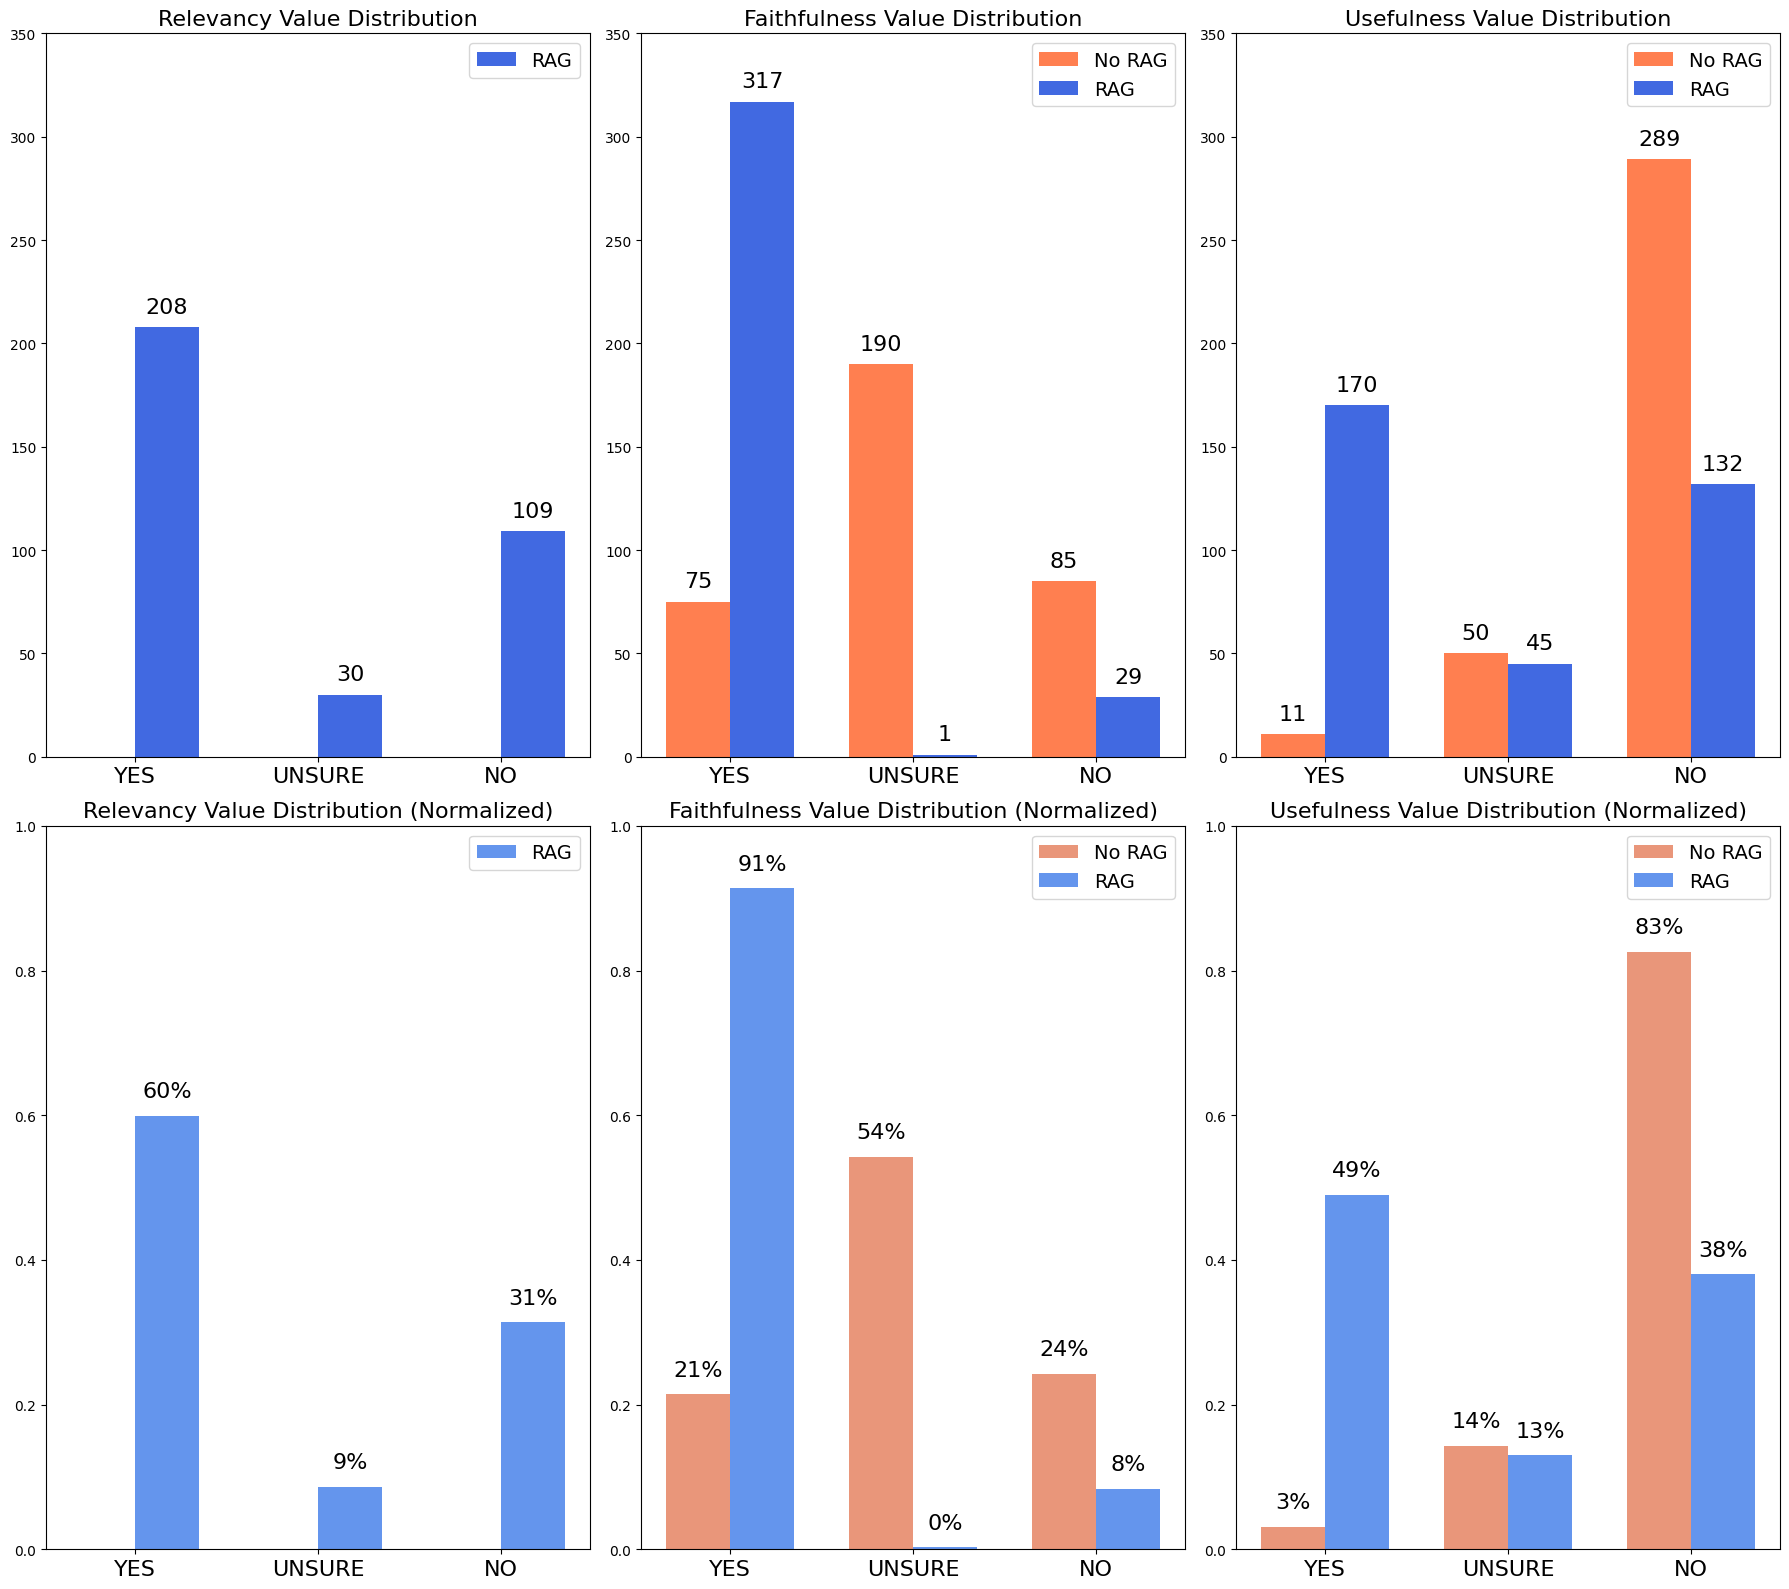
\includegraphics[width=\textwidth,height=\textheight,keepaspectratio]{Figures/RegularQA_res.png}
\caption{The results of the Regular Questions set experiments}
\label{fig:RegularQA_res}
\end{figure}

As can be seen, the use of context (RAG setup) in the system does indeed significantly improve the quality of LLM responses.

We can then analyze in more detail the results of the metrics in terms of each question. The task does not require an absolutely precise approach, but a distribution of averages is sufficient. For this purpose, the assessment results were converted into scores: 0 for “No”, 0.5 for “Unsure”, and 1 for “Yes”. Further, to visualize the results, a heatmap was constructed, which shows the distribution of results by questions. The results are illustrated in the heatmap in the \autoref{fig:results_heatmap}:
\begin{figure}[H]
\centering
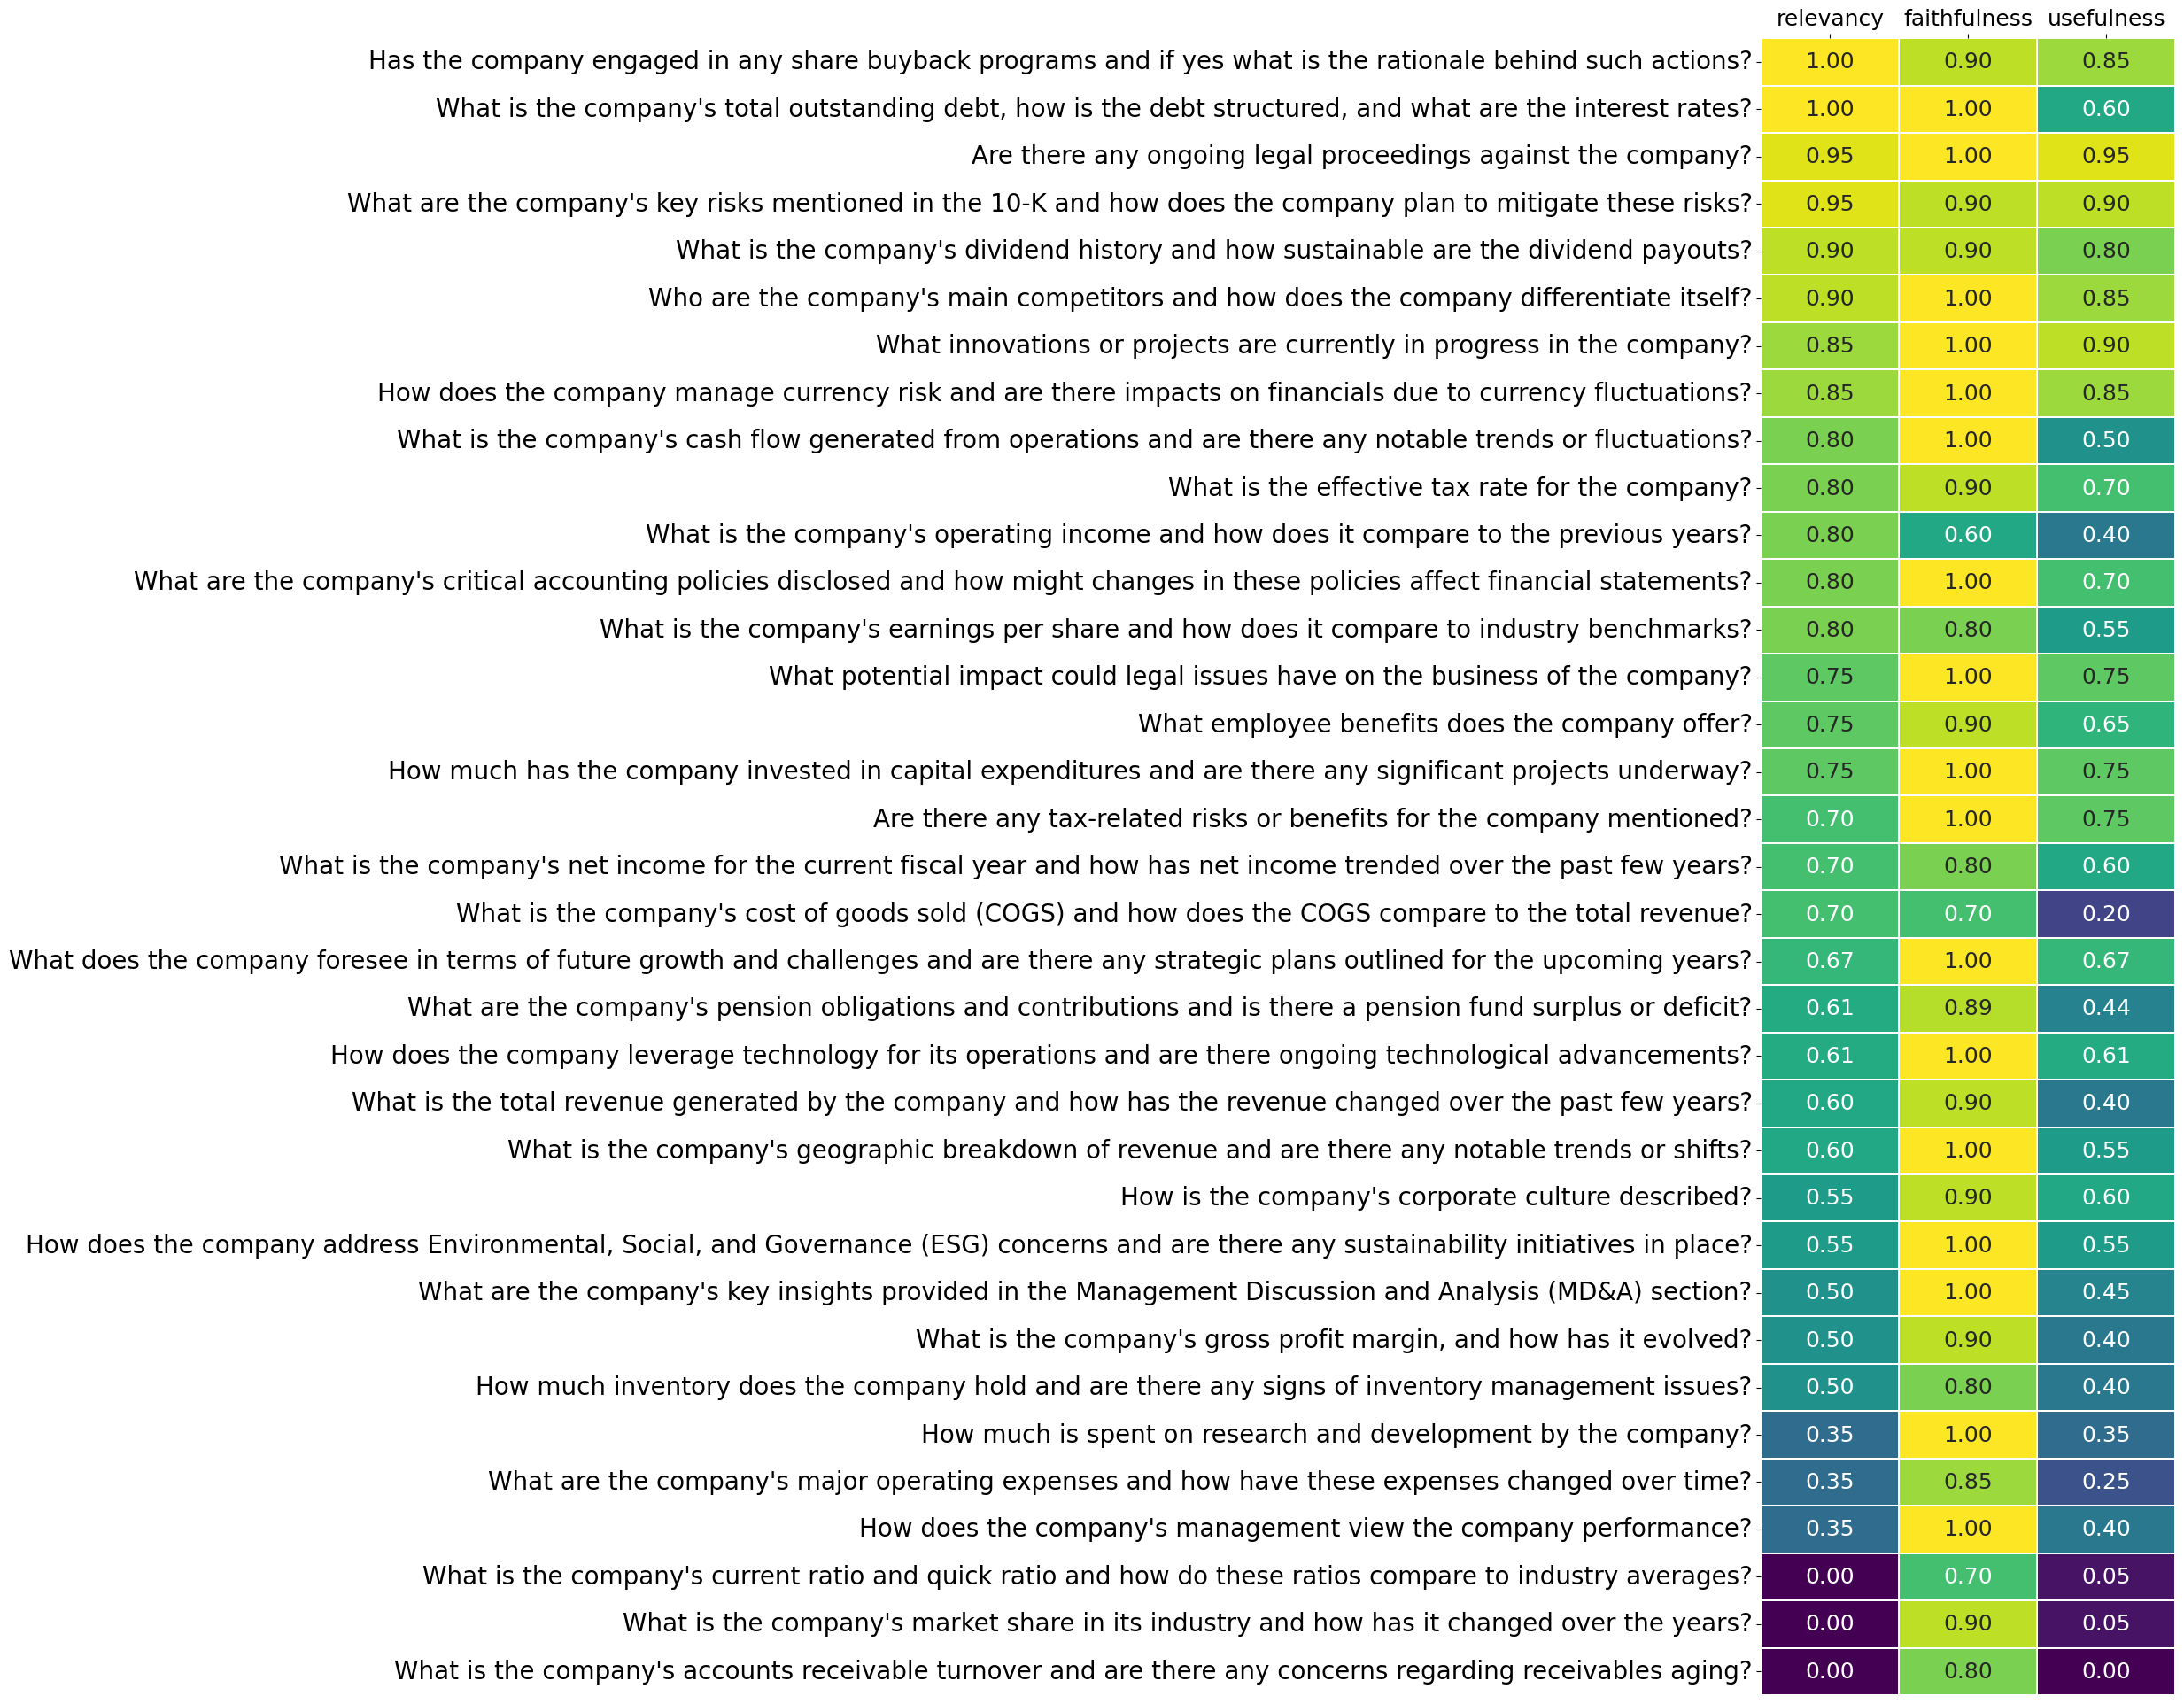
\includegraphics[width=1\textwidth]{Figures/results_heatmap.png}
\caption{The heatmap for the questions accuracy results of the Regular Questions dataset experiments}
\label{fig:results_heatmap}
\end{figure}
\\
The heatmap presents the average relevancy, faithfulness, and usefulness values for each query in the Regular Questions dataset. These metrics provide a quantifiable measure of the quality of the responses generated by the model.

Most queries exhibit high relevancy and faithfulness scores, particularly those related to direct financial information and strategic insights. Queries like "Has the company engaged in any share buyback programs and if yes what is the rationale behind such actions?" and "What is the company's total outstanding debt, how is the debt structured, and what are the interest rates?" scored perfect relevancy and near-perfect faithfulness.

Usefulness scores are more varied compared to relevancy and faithfulness. Some queries with high relevancy and faithfulness still show moderate usefulness, suggesting either that while the responses are accurate and relevant they might lack practical application or depth, or that the responses are not accurate at all. For instance, the query "What is the company's total outstanding debt, how is the debt structured, and what are the interest rates?" has high relevancy and faithfulness but a moderate usefulness score of 0.6.

Certain queries have notably low scores across all metrics. For example, "What is the company's current ratio and quick ratio and how do these ratios compare to industry averages?" shows zero relevancy and usefulness, indicating a significant gap in the model's ability to address this type of question. Queries related to market share and accounts receivable turnover also score very low, suggesting the need for improved data retrieval or response generation strategies for these topics. 

Some queries maintain a balanced performance across all metrics, such as "What are the company's key risks mentioned in the 10-K and how does the company plan to mitigate these risks?", which shows high scores in relevancy (0.95), faithfulness (0.9), and usefulness (0.9).

Main conclusions and insights about the Regular Questions set experiments results:
\begin{enumerate}
\item The RAG pipeline performs well in retrieving and generating relevant, faithful, and useful answers for questions related to financial metrics, corporate structure, and competitive analysis.
\item The pipeline struggles with more subjective or complex queries, such as those related to market share, management perspectives, and future growth predictions.
\item Evaluating outcomes is challenging due to the absence of ground truth values for comparison. Thus, we are essentially measuring precision without the ability to measure recall.
\item Some LLM responses include data from the given context but erroneously apply it to other indicators.
\item Some questions lack the necessary information for an answer. In these cases, the retrieved context is evaluated as irrelevant, leading to no distinction between reports that do not contain the information at all and those where retrieval provided an irrelevant document.
\item The "Key Risks" section in reports is often lengthy, containing several pages describing possible risks. The RAG chain is limited by the number of contexts set by the hyperparameter "NUM\_CHUNKS" (set to 2 in our experiments) and by the LLM context window (4,000 tokens for the Phi-3 model). This limitation affects the quality of the final response, typically resulting in the LLM response covering only part of the necessary information.
\end{enumerate}

\subsubsection{Evaluation and Results for the FinanceBench questions set}
A second evaluation was conducted on the FinanceBench Questions set, which comprises 150 questions. For the FinanceBench Questions set the questions, retrieved context (whether relevant or irrelevant to the question), generated responses and ground truth answers were saved as a CSV file. This dataset was then uploaded to the Argilla workspace (a framework that utilizes HuggingFace space) for manual annotation. The dataset was evaluated using the following metrics, with set of ["YES", "NO", "UNSURE"] possible answers for each question:
\begin{enumerate}
\item Usefulness metric. The answer to the question "Is generated answer useful to resolve a question?". If the answer is incorrect or irrelevant, it is not useful. If the response merely indicates where the requested data can be obtained, it is considered unhelpful. A 'YES' for the 'usefulness' metric indicates correct answers or answers containing some correct information. 'NO' also includes factually incorrect answers and responses where the context does not contain relevant information, and the LLM's answer is simply "I do not know" or "I do not have specific information".
\item Correctness metric. The answer to the question "Does the generated answer match the ground truth answer?". The Financebench dataset provides the correct (ground truth) answers to the question. When answering the question, the correct (ground truth) answer was compared to the answer provided by the system.
\end{enumerate}

After all the results of the experiments with FinanceBench Questions set were evaluated on Argilla workspace, the results were analyzed. The distribution of responses between the metrics is shown in the \autoref{table:comparison_FB}:
\begin{table}[H]
\centering
\begin{tabular}{|c|c|c|c|c|}
\hline
\textbf{Metric} & \textbf{Setup} & \textbf{YES} & \textbf{UNSURE} & \textbf{NO} \\ 
\hline
\multirow{2}{*}{Usefulness} & No RAG & 10 (7\%) & 8 (5\%) & 132 (88\%) \\ \cline{2-5}
 & RAG & 25 (17\%) & 15 (10\%) & 110 (73\%) \\
\hline
\multirow{2}{*}{Correctness} & No RAG & 7 (5\%) & 15 (10\%) & 128 (85\%) \\ \cline{2-5}
 & RAG & 20 (13\%) & 11 (7\%) & 119 (79\%) \\
\hline
\end{tabular}
\caption{Comparison of Usefulness and Correctness between No\_RAG and RAG setups}
\label{table:comparison_FB}
\end{table}
The RAG system improves the correctness (from 5\% with No RAG setup to 13\% with RAG setup) and usefulness (from 7\% without RAG to 17\% with RAG) of the LLM-generated answers.

The distribution of the results are shown in the \autoref{fig:results_financebench150}:
\begin{figure}[H]
\centering
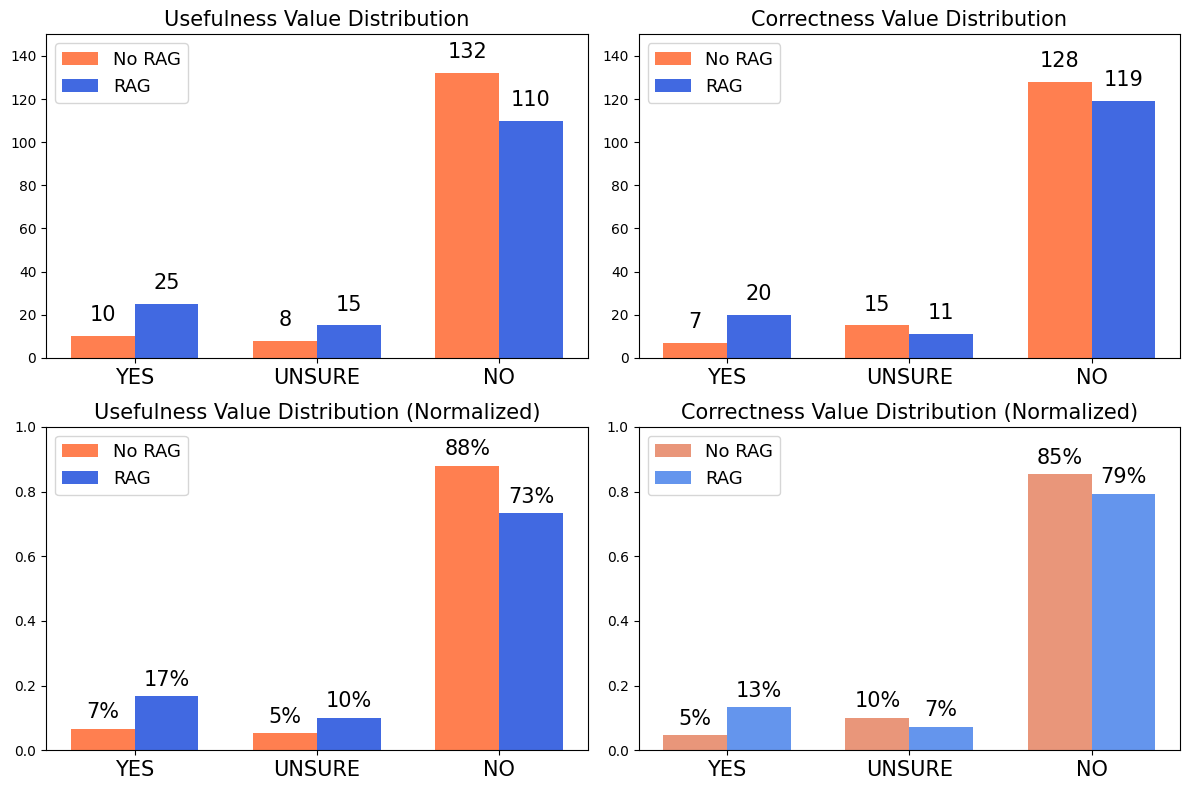
\includegraphics[width=1\textwidth]{Figures/results_financebench150.png}
\caption{The results of the Financebench Questions set experiments}
\label{fig:results_financebench150}
\end{figure}

Without access to additional information (No RAG setup), in a closed book configuration, LLM performs poorly on the Financebench Questions set, phi-3-mini model only gives correct answers to 5\% of questions (the GPT-4-Turbo model in the same closed book configuration gives correct answers to 9\% of prompts \cite{Islam.20Nov2023}), and in a RAG configuration the results are up to 13\%.

The results of the experiments show that 86\% of answers with RAG setup were incorrect (total 'UNSURE' and 'NO' answers), which is very similar to the results obtained by the authors of the Financebench paper with state-of-the-art models. According to the Financebench paper authors tested different LLM configurations including GPT-4-Turbo, Llama2, and Claude2, with and without vector stores and long context prompts, on a FinanceBench questions set and manually reviewed their answers. The best results are from GPT-4-Turbo in oracle setup (with access to evidence pages of the financial reports) with 85\% accuracy. But such a system is impossible in real life. The same GPT-4-Turbo with long context (the whole report was provided to the LLM as context) setup has 79\% accuracy. Single vector store (one vector database for each report) with GPT-4-Turbo has 50\% correct answers, and with Llama 2 - 41\%. And shared vector store systems (one vectorbase for all reports) with both GPT-4-Turbo and Llama 2 models have the same accuracy of 19\%. Existing LLMs have clear limitations for financial questions \cite{Islam.20Nov2023}. 

The RAG pipeline shows the worst results (lowest precision) when answering questions that contain complex queries or multiple sub-questions, especially when the terms are not present in the reports. At the same time if the presented context is of high quality the RAG pipeline is capable of formulating answers to complex queries. In most cases, the reason for an answer being useless is the lack of specific information needed to respond. These indicate that the retrieval stage is crucial for the system's overall performance.

RAG setup helps in answering financial questions, but introduces many related problems, particularly with reasoning. RAG functions well as a search engine, but not as a definitive source of answers. It seems that end-to-end answering of questions is not feasible at this stage. For a RAG system, it is very difficult to capture all important references from a question.